% tesesusp.cls, v-0.0.1

% Based on 'bntex2ppgsi.cls', 'abntex2.csl' and on USP guidelines to create
% thesis and dissertation documents.
% See <https://www.overleaf.com/project/64f7bdf1641ad4a3a8482800>
% and <https://teses.usp.br/index.php?option=com_content&
%      view=article&id=52&Itemid=67&lang=en>
% to learn more.

\clearpage

%:::% class attribute begin/end %:::%

% ----------------------------------------------------------------------
% Cover (mandatory)
% ----------------------------------------------------------------------

%:::% cover body-tag begin %:::%
\imprimircapa
%:::% cover body-tag end %:::%

% ----------------------------------------------------------------------
% Title page (mandatory)
% ----------------------------------------------------------------------

%:::% approval-sheet body-tag begin %:::%
\imprimirfolhaderosto*
%:::% approval-sheet body-tag end %:::%

% ----------------------------------------------------------------------
% Cataloging record (mandatory)
% ----------------------------------------------------------------------

%:::% cataloging-record begin %:::%
\begin{fichacatalografica}
 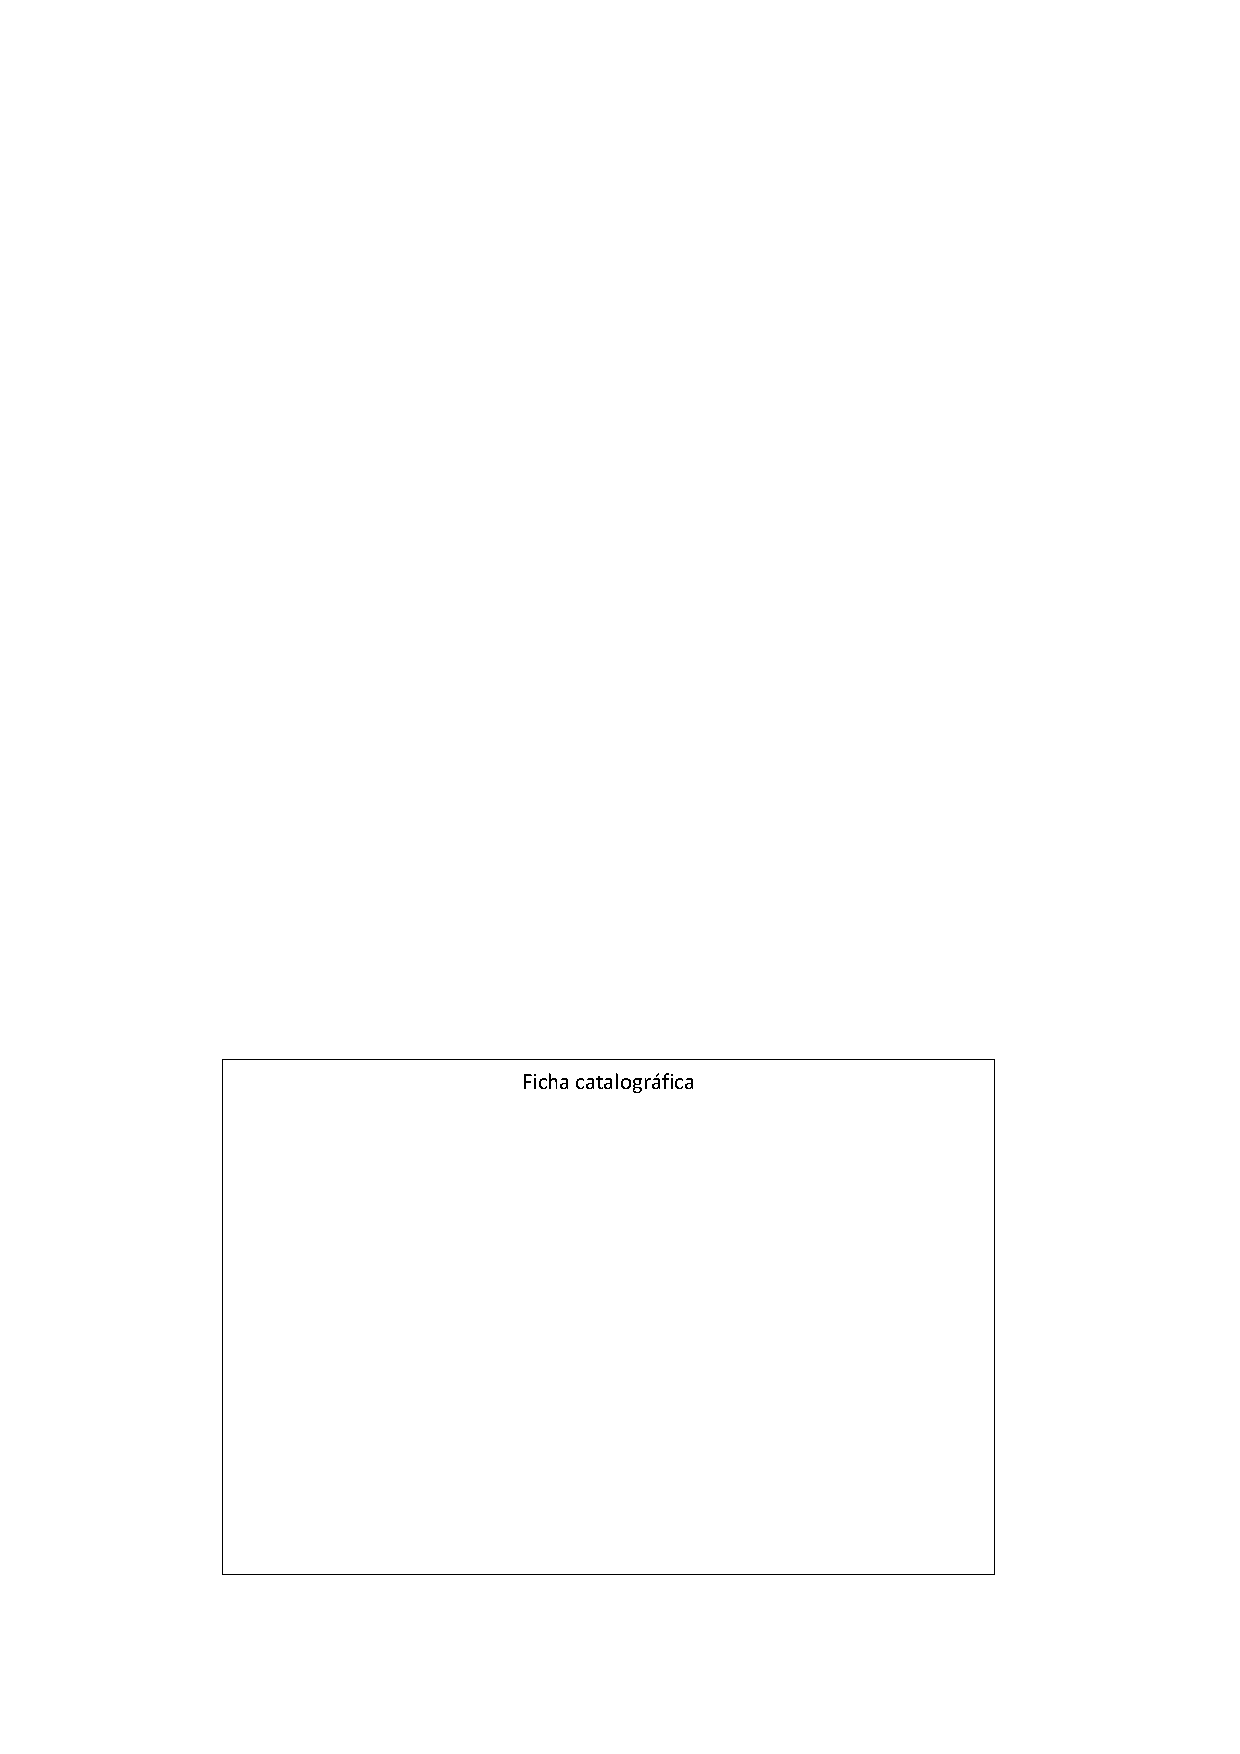
\includepdf{images/fig_ficha_catalografica.pdf}
\end{fichacatalografica}
%:::% cataloging-record end %:::%

% ----------------------------------------------------------------------
% Errata (optional)
% ----------------------------------------------------------------------

%:::% errata begin %:::%
\begin{errata}
  %:::% errata body begin %:::%
This is the development version of the thesis (version \textless1.0.0).
Any necessary corrections will be listed here after its approval.
  %:::% errata body end %:::%
\end{errata}
%:::% errata end %:::%

% ----------------------------------------------------------------------
% Approval sheet (mandatory)
% ----------------------------------------------------------------------

%:::% approval-sheet begin %:::%
\begin{folhadeaprovacao}
  \noindent
  %:::% approval-sheet header begin %:::%
{[}TYPE OF WORK{]} by {[}AUTHOR'S FULL NAME{]}, under the title
\textbf{\{tesesusp\}: a Quarto format for USP theses and dissertations},
presented to the {[}SCHOOL/DEPARTMENT{]} at the University of São Paulo,
as part of the requirements for the degree of {[}TYPE OF DEGREE{]} by
the {[}GRADUATE PRGRAM{]}), in the concentration area of
{[}CONCENTRATION AREA{]}.
  %:::% approval-sheet header end %:::%

  \vspace*{1.5cm}

  \noindent
  Approved on \_\_\_\_\_\_\_\_\_\_\_\_\_\_\_\_\_\_\_\_ , \_\_\_\_\_\_\_\_\_\_ .

  \vspace*{1.5cm}

  \begin{center}
    \noindent Examination committee
  \end{center}

  \vspace*{0.5cm}

  \noindent Committee chair:

  \vspace*{0.25cm}

  \renewcommand{\arraystretch}{2}
  \setlength{\arrayrulewidth}{0pt}
  \setlength{\tabcolsep}{0pt}
  \noindent
  \begin{tabular}{m{2cm} P{14cm}}
    Prof. Dr. & \_\_\_\_\_\_\_\_\_\_\_\_\_\_\_\_\_\_\_\_\_\_\_\_\_\_\_\_\_\_\_\_\_\_\_\_\_\_\_\_\_\_\_\_\_\_\_\_\_\_\_\_\_\_\_ \\
    Institution & \_\_\_\_\_\_\_\_\_\_\_\_\_\_\_\_\_\_\_\_\_\_\_\_\_\_\_\_\_\_\_\_\_\_\_\_\_\_\_\_\_\_\_\_\_\_\_\_\_\_\_\_\_\_\_ \\
  \end{tabular}

  \vspace*{1cm}

  \noindent Examiners:

  \vspace*{0.25cm}

  \noindent
  \begin{tabular}{m{2cm} P{14cm}}
    Prof. Dr. & \_\_\_\_\_\_\_\_\_\_\_\_\_\_\_\_\_\_\_\_\_\_\_\_\_\_\_\_\_\_\_\_\_\_\_\_\_\_\_\_\_\_\_\_\_\_\_\_\_\_\_\_\_\_\_ \\
    Institution & \_\_\_\_\_\_\_\_\_\_\_\_\_\_\_\_\_\_\_\_\_\_\_\_\_\_\_\_\_\_\_\_\_\_\_\_\_\_\_\_\_\_\_\_\_\_\_\_\_\_\_\_\_\_\_ \\
    Evaluation & \_\_\_\_\_\_\_\_\_\_\_\_\_\_\_\_\_\_\_\_\_\_\_\_\_\_\_\_\_\_\_\_\_\_\_\_\_\_\_\_\_\_\_\_\_\_\_\_\_\_\_\_\_\_\_ \\
  \end{tabular}

  \vspace*{0.5cm}

  \noindent
  \begin{tabular}{m{2cm} P{14cm}}
    Prof. Dr. & \_\_\_\_\_\_\_\_\_\_\_\_\_\_\_\_\_\_\_\_\_\_\_\_\_\_\_\_\_\_\_\_\_\_\_\_\_\_\_\_\_\_\_\_\_\_\_\_\_\_\_\_\_\_\_ \\
    Institution & \_\_\_\_\_\_\_\_\_\_\_\_\_\_\_\_\_\_\_\_\_\_\_\_\_\_\_\_\_\_\_\_\_\_\_\_\_\_\_\_\_\_\_\_\_\_\_\_\_\_\_\_\_\_\_ \\
    Evaluation & \_\_\_\_\_\_\_\_\_\_\_\_\_\_\_\_\_\_\_\_\_\_\_\_\_\_\_\_\_\_\_\_\_\_\_\_\_\_\_\_\_\_\_\_\_\_\_\_\_\_\_\_\_\_\_ \\
  \end{tabular}

  \vspace*{0.5cm}

  \noindent
  \begin{tabular}{m{2cm} P{14cm}}
    Prof. Dr. & \_\_\_\_\_\_\_\_\_\_\_\_\_\_\_\_\_\_\_\_\_\_\_\_\_\_\_\_\_\_\_\_\_\_\_\_\_\_\_\_\_\_\_\_\_\_\_\_\_\_\_\_\_\_\_ \\
    Institution & \_\_\_\_\_\_\_\_\_\_\_\_\_\_\_\_\_\_\_\_\_\_\_\_\_\_\_\_\_\_\_\_\_\_\_\_\_\_\_\_\_\_\_\_\_\_\_\_\_\_\_\_\_\_\_ \\
    Evaluation & \_\_\_\_\_\_\_\_\_\_\_\_\_\_\_\_\_\_\_\_\_\_\_\_\_\_\_\_\_\_\_\_\_\_\_\_\_\_\_\_\_\_\_\_\_\_\_\_\_\_\_\_\_\_\_ \\
  \end{tabular}
\end{folhadeaprovacao}
%:::% approval-sheet end %:::%

% ----------------------------------------------------------------------
% Inscription (optional)
% ----------------------------------------------------------------------

%:::% inscription begin %:::%
\begin{dedicatoria}
  \vspace*{\fill}
  \centering
  %:::% inscription body begin %:::%
\emph{To the worm that first gnawed on the cold flesh of my corpse,}

\emph{I dedicate, as a fond remembrance, these posthumous memories.}

\vspace{1cm}

Inscription found in the book

\emph{The Posthumous Memoirs of Brás Cubas} by Machado de Assis (2014).
  %:::% inscription body end %:::%
	\vspace*{\fill}
\end{dedicatoria}
%:::% inscription end %:::%

% ----------------------------------------------------------------------
% Acknowledgments (optional)
% ----------------------------------------------------------------------

%:::% acknowledgments begin %:::%
\begin{agradecimentos}
  %:::% acknowledgments body begin %:::%
I would like to acknowledge this awesome
\href{https://github.com/danielvartan/tesesusp}{Quarto format}! :)
  %:::% acknowledgments body end %:::%
\end{agradecimentos}
%:::% acknowledgments end %:::%

% ----------------------------------------------------------------------
% Epigraph (optional)
% ----------------------------------------------------------------------

%:::% epigraph begin %:::%
\begin{epigrafe}
  \vspace*{\fill}
	\begin{flushright}
	  %:::% epigraph body begin %:::%
\emph{Nullius in verba}

(The Royal Society, n.d.)
		%:::% epigraph body end %:::%
	\end{flushright}
\end{epigrafe}
%:::% epigraph end %:::%

% ----------------------------------------------------------------------
% Abstract in the vernacular language (mandatory)
% ----------------------------------------------------------------------

%:::% vernacular-abstract begin %:::%
\setlength{\absparsep}{18pt}
\begin{resumo}
  %:::% vernacular-abstract body begin %:::%
{[}SURNAME{]}, {[}INITIALS{]}. ({[}YEAR{]}). \emph{{[}TITLE{]}}
{[}{[}TYPE OF THESIS{]}{]}. {[}SCHOOL/DEPARTMENT{]}, University of São
Paulo, São Paulo. {[}THESIS'S URL{]}

Cupidatat ad culpa non veniam quis mollit dolor ut irure eiusmod sint
aute duis. Mollit eu ipsum deserunt nisi est culpa exercitation dolor.
Velit veniam ad elit aliqua excepteur consectetur duis cillum id do
mollit dolor pariatur aute. Excepteur velit ea aliqua amet fugiat qui
aliquip tempor. Labore occaecat mollit minim in velit est nisi. Ut
voluptate laboris ad amet culpa excepteur voluptate eiusmod est.
Adipisicing eu fugiat irure sunt id tempor consectetur sint ipsum
cillum. Ex sunt enim anim quis cupidatat reprehenderit reprehenderit
nisi ea amet. Ullamco minim voluptate tempor nostrud id voluptate
exercitation. Elit sint ea occaecat ipsum dolore incididunt velit
cupidatat id. Consectetur aliquip dolore elit aute elit et ex ex fugiat
ex laboris non magna. Duis voluptate mollit laborum aliquip elit mollit
ad nisi sunt id ipsum esse incididunt eiusmod. Qui incididunt
consectetur cillum est ex proident ad eiusmod excepteur pariatur velit
enim ut cillum. Fugiat exercitation veniam eiusmod irure ut ad sint sunt
consequat consectetur. Dolor sint voluptate mollit anim dolor ea ad ex
veniam.

Keywords: keyword 1. keyword 2. keyword 3.
  %:::% vernacular-abstract body end %:::%
\end{resumo}
%:::% vernacular-abstract end %:::%

% ----------------------------------------------------------------------
% Abstract in the foreign language (mandatory)
% ----------------------------------------------------------------------

%:::% foreign-abstract begin %:::%
\begin{resumo}[RESUMO]
  \begin{otherlanguage*}{brazil}
    %:::% foreign-abstract body begin %:::%
{[}SOBRENOME{]}, {[}INICIAIS{]}. ({[}ANO{]}). \emph{{[}TÍTULO{]}}
{[}{[}TIPO DE TESE/DISSERTAÇÃO{]}{]}. {[}ESCOLA/DEPARTAMENTO{]},
Universidade de São Paulo, São Paulo. {[}URL DA DISSERTAÇÃO/TESE{]}

Cillum qui eu non ipsum pariatur ad exercitation pariatur dolore veniam
amet cillum. Aliqua do nostrud aliquip in amet. Commodo sit tempor nulla
ipsum officia voluptate laborum elit minim proident Lorem. Id pariatur
reprehenderit non officia fugiat incididunt anim aliquip anim anim.
Ipsum irure magna quis est aute. Nostrud nulla mollit non labore. In
laboris mollit ea in. Excepteur eu do elit proident. Commodo tempor nisi
enim ex velit voluptate dolor mollit eiusmod in ullamco aliqua nostrud
id. Eiusmod dolore sint proident consectetur reprehenderit exercitation
sunt. Nisi qui sit commodo anim consectetur in laborum dolore in labore
veniam labore commodo tempor. Sunt sit officia commodo quis magna.
Aliqua esse est adipisicing ea est ex esse esse officia sit culpa minim
amet dolore. Culpa dolore laborum sunt do commodo duis in velit. Mollit
duis voluptate aliquip magna labore aute sit dolore amet culpa labore.
Id tempor consectetur est anim ullamco ex nostrud voluptate excepteur.
Aliqua laboris aute laborum amet eu. Minim quis veniam et dolor quis
fugiat. Adipisicing amet est do aliqua nostrud amet excepteur ut.

Palavras-chaves: palavra-chave 1. palavra-chave 2. palavra-chave 3.
    %:::% foreign-abstract body end %:::%
  \end{otherlanguage*}
\end{resumo}
%:::% foreign-abstract end %:::%

% ----------------------------------------------------------------------
% List of figures (optional)
% ----------------------------------------------------------------------

%:::% list-of-figures begin %:::%
\renewcommand{\listfigurename}{LIST OF FIGURES}
\pdfbookmark[0]{\listfigurename}{lof}
\listoffigures*
\cleardoublepage
%:::% list-of-figures end %:::%

% ----------------------------------------------------------------------
% List of tables (optional)
% ----------------------------------------------------------------------

%:::% list-of-tables begin %:::%
\renewcommand{\listtablename}{LIST OF TABLES}
\pdfbookmark[0]{\listtablename}{lot}
\listoftables*
\cleardoublepage
%:::% list-of-tables end %:::%

% ----------------------------------------------------------------------
% List of abbreviations and acronyms (optional)
% ----------------------------------------------------------------------

%:::% list-of-abbreviations begin %:::%
\begin{siglas}
  %:::% list-of-abbreviations body begin %:::%
\begin{description}
\item[\textsubscript{F}]
\hspace{20cm}

Subscript indicating a relation with work-free days.
\item[\textsubscript{W}]
\hspace{20cm}

Subscript indicating a relation with workdays.
\item[MCTQ]
\hspace{20cm}

Munich ChronoType Questionnaire.
\item[MCTQ\textsuperscript{PT}]
\hspace{20cm}

Portuguese version of the MCTQ.
\item[MEQ]
\hspace{20cm}

Morningness-Eveningness Questionnaire
\item[MSF]
\hspace{20cm}

Local time of mid-sleep on work-free days.
\item[MSF\textsubscript{sc}]
\hspace{20cm}

Chronotype proxy. The midpoint between sleep onset and sleep end on
work-free days. A sleep correction (\textsubscript{SC}) is made when a
possible sleep compensation related to a lack of sleep on workdays is
identified.
\item[MSW]
\hspace{20cm}

Local time of mid-sleep on workdays.
\end{description}
  %:::% list-of-abbreviations body end %:::%
\end{siglas}
%:::% list-of-abbreviations end %:::%

% ----------------------------------------------------------------------
% List of symbols (optional)
% ----------------------------------------------------------------------

%:::% list-of-symbols begin %:::%
\begin{simbolos}
  %:::% list-of-symbols body begin %:::%
For an extensive list of chronobiology terms and definitions, please
refer to Aschoff et al.~(1965) and Marques \& Oda (2012).

\begin{description}
\item[\(\tau\)]
\hspace{20cm}

Period of a rhythm in free flow; only revealed under constant
environmental conditions.
\item[\(T\)]
\hspace{20cm}

Zeitgeber period.
\item[\(\phi\)]
\hspace{20cm}

Phase
\item[\(\Delta\phi\)]
\hspace{20cm}

Phase shift
\item[\(+\Delta\phi\)]
\hspace{20cm}

Phase advance
\item[\(-\Delta\phi\)]
\hspace{20cm}

Phase delay
\item[\(\Psi\)]
\hspace{20cm}

Phase relation
\end{description}
  %:::% list-of-symbols body end %:::%
\end{simbolos}
%:::% list-of-symbols end %:::%

% ----------------------------------------------------------------------
% List of terms and definitions (optional)
% ----------------------------------------------------------------------

%:::% list-of-terms begin %:::%
\begin{termos}
  %:::% list-of-terms body begin %:::%
For an extensive list of chronobiology terms and definitions, please
refer to Aschoff et al.~(1965) and Marques \& Oda (2012).

\begin{description}
\item[Chronotype]
\hspace{20cm}

Any kind of temporal phenotype (Ehret, 1974; Pittendrigh, 1993).
Usually, it refers to circadian phenotypes in a spectrum that goes from
morningness to eveningness (Horne \& Ostberg, 1976; Roenneberg et al.,
2003). It can also be seen as an organism's phase of entrainment
(Roenneberg et al., 2012).
\end{description}

\begin{description}
\item[Circadian rhythm]
\hspace{20cm}

A rhythm with a period close to a day/24h, an approximation to the
period of the earth's rotation (Pittendrigh, 1960). From the Latin
\emph{circā}, around, and \emph{dĭes}, day (Latinitium, n.d.). Example:
the sleep-wake cycle.
\end{description}

\begin{description}
\item[Complex system]
\hspace{20cm}

There are several definitions. Here are some that I found to be of use:
\end{description}

\begin{itemize}
\tightlist
\item
  ``Systems that don't yield to compact forms of representation or
  description.'' (David Krakauer apud Mitchell, 2013)
\item
  ``A system of many interacting parts where the system is more than
  just the sum of its parts'' (Mark Newman apud Mitchell, 2013)
\item
  Systems with many connected agents that interact and exhibit
  self-organization and emergence behavior, all without the need for a
  central controller (adapted from Camilo Rodrigues Neto's definition,
  supervisor of this thesis).
\item
  Dialectics at its finest (my working definition).
\end{itemize}

\begin{description}
\item[Entrainment]
\hspace{20cm}

A shift and alignment of biological rhythms induced by a zeitgeber input
(Kuhlman et al., 2018). For example: a shift/alignment of an organism's
circadian rhythm when exposed to light.
\end{description}

\begin{description}
\item[Infradian rhythm]
\hspace{20cm}

A rhythm with a period greater than a day/24h. From the Latin
\emph{infrā}, below (think in terms of period repetition), and
\emph{dĭes}, day (Latinitium, n.d.). Example: the menstrual cycle.
\end{description}

\begin{description}
\item[Period]
\hspace{20cm}

Cycle duration of an oscillation or, in a more technical way, the
duration between two identical and consecutive phases in an oscillation
(Kuhlman et al., 2018).
\end{description}

\begin{description}
\item[System theory]
\hspace{20cm}

Two definitions can be of use:
\end{description}

\begin{itemize}
\tightlist
\item
  Science or discipline that investigates models, principles, and laws
  that are valid to systems in general (Bertalanffy, 1968).
\item
  ``The attempt of a reductionist scientific tradition to come to terms
  with complexity, nonlinearity, and change through sophisticated
  mathematical and computational techniques, \emph{a groping toward a
  more dialectical understanding} that is held back by its philosophical
  biases and the institutional and economic contexts of its
  development.'' (Levins, 1998)
\end{itemize}

\begin{description}
\item[Ultradian rhythm]
\hspace{20cm}

A rhythm with a period below a day/24h. From the Latin \emph{ultrā},
beyond (think in terms of period repetition), and \emph{dĭes}, day
(Latinitium, n.d.). Example: the cardiac cycle.
\end{description}

\begin{description}
\item[Zeitgeber]
\hspace{20cm}

Any periodic environmental signal/cue that can influence or regulate
biological rhythms. From the German \emph{zeit}, time, and \emph{geber},
donor (Cambridge University Press, n.d.). Two main well known zeitgebers
are light exposure and environment temperature (Pittendrigh, 1960).
\end{description}
  %:::% list-of-terms body end %:::%
\end{termos}
%:::% list-of-terms end %:::%

% ----------------------------------------------------------------------
% Table of contents (mandatory)
% ----------------------------------------------------------------------

%:::% table-of-contents begin %:::%
\renewcommand{\contentsname}{TABLE OF CONTENTS}
\pdfbookmark[0]{\contentsname}{toc}
% \tableofcontents*
\cleardoublepage
%:::% table-of-contents end %:::%
